\pdfminorversion=7
\DeclareUnicodeCharacter{2212}{-}
\documentclass{beamer}
\usepackage[utf8]{inputenc}
\usepackage{siunitx}
\usepackage{amsmath}
\usepackage{slashed}
\usepackage{fancyvrb}
\usepackage{epstopdf}
\usepackage{xcolor}
\hypersetup{
    colorlinks=true,
    linkcolor=blue,
    filecolor=magenta,      
    urlcolor=cyan,
}
\usetheme{boxes}
\newcommand{\ks}{\ensuremath{K_S^0}}
\newcommand{\strphdiff}{\ensuremath{\Delta \delta_D}}
\newcommand{\kspipi}[1]{\ensuremath{#1 \to \ks \pi^+ \pi^-}}
\newcommand{\diffDtokspipi}{\ensuremath{\kspipi{D^0}} \text{and} \ensuremath{\kspipi{\bar{D}^0}} }
\newcommand{\MP}{\ensuremath{m^2_+}}
\newcommand{\MM}{\ensuremath{m^2_-}}
\newcommand{\MZ}{\ensuremath{m^2_0}}
\newcommand{\phasePosition}{\ensuremath{m^2_+,m^2_-}}
\newcommand{\phasePositionT}{\ensuremath{m^2_-,m^2_+}}
\newcommand{\Dzbar}{\ensuremath{\bar{D}^0} }
\newcommand{\Dz}{\ensuremath{D^0} }
\newcommand{\Bzbar}{\ensuremath{\bar{B}^0} }
\newcommand{\Bz}{\ensuremath{B^0} }
%These macros are save time, usage
%\subAmp{particle}{component} -e.g \subAmp{\Dz}{L_{\pi^+\pi^-}=0}
\newcommand{\subAmp}[2]{\ensuremath{A_{#1}^{#2}\left(\phasePosition \right)}}
%\modelAmp{particle}{model name} - e.g. \modelAmp{\Dz}{Belle}
\newcommand{\modelAmp}[2]{\ensuremath{A_{#1}^{\text{#2}}\left(\phasePosition \right)}}
\newcommand{\genAmp}[2]{\ensuremath{A_{#1}^{\text{#2}}\left(\mathcal{P} \right)}}
%Generic input amp (actually you could use \modelAmp instead if you want
\newcommand{\inputAmp}[1]{\ensuremath{A_{#1}^{\text{input}}\left(\phasePosition\right)}}
%True model - what the decay really is
\newcommand{\trueAmp}[1]{\ensuremath{A_{#1}^{\text{True}}\left(\phasePosition\right)}}
%a_r and phi_r, again saves writing $, _, ^ everywhere
\newcommand{\magPar}[1]{\ensuremath{a_{#1}}}
\newcommand{\phPar}[1]{\ensuremath{\phi_{#1}}}
\author{Jake Lane}
\title{Individual Resonances for the Belle Model}
\begin{document}


\begin{frame}{Introduction}
We perform a ``Self Fit'' for two particular models (``myBelle'' and ``timBelle''). 
The purpose of this is to establish a ``baseline'' fit for a given model.
\end{frame}
\begin{frame}{Procedure}
The ``SelfFit'' Procedure is
\begin{itemize}
\item Generate a toy MC sample, $\mathcal{G}$ from a given model, $\mathcal{M}$
\item Fit $\mathcal{G}$ using the same model, $\mathcal{M}$ and obtain a ``fitted'' model, $\mathcal{M}'$
\item Regenerate another toy sample, $\mathcal{G}'$ from this ``new'' model, $\mathcal{M}'$
\end{itemize}
\end{frame}

\begin{frame}{\MP for Belle\ Model\ (Tim)}
\begin{columns}[t]
\column{0.5\textwidth}
\centering
\includegraphics[width=.7\linewidth]{output/timBelle/D0//regenerated/s01.png}
\column{0.5\textwidth}
\centering
\includegraphics[width=.7\linewidth]{output/timBelle/D0//fitted/s01.png}
\end{columns}
    \centering
    Left ``Regenerated Model'', right ``Original Model (with fit line)''
\end{frame}                   

\begin{frame}{\MM for Belle\ Model\ (Tim)}
\begin{columns}[t]
\column{0.5\textwidth}
\centering
\includegraphics[width=.7\linewidth]{output/timBelle/D0//regenerated/s02.png}
\column{0.5\textwidth}
\centering
\includegraphics[width=.7\linewidth]{output/timBelle/D0//fitted/s02.png}
\end{columns}
    \centering
    Left ``Regenerated Model'', right ``Original Model (with fit line)''
\end{frame}                   

\begin{frame}{\MZ for Belle\ Model\ (Tim)}
\begin{columns}[t]
\column{0.5\textwidth}
\centering
\includegraphics[width=.7\linewidth]{output/timBelle/D0//regenerated/s12.png}
\column{0.5\textwidth}
\centering
\includegraphics[width=.7\linewidth]{output/timBelle/D0//fitted/s12.png}
\end{columns}
    \centering
    Left ``Regenerated Model'', right ``Original Model (with fit line)''
\end{frame}                   


\begin{frame}{\MP vs \MM for Belle\ Model\ (Tim)}
\begin{columns}[t]
\column{0.5\textwidth}
\centering
\includegraphics[width=.7\linewidth]{output/timBelle/D0//regenerated/s01_vs_s02.png}
\column{0.5\textwidth}
\centering
\includegraphics[width=.7\linewidth]{output/timBelle/D0//initial/s01_vs_s02.png}
\end{columns}
    \centering
    Left ``Regenerated'', right ``Original''
\end{frame} 


\begin{frame}{\MP vs \MZ for Belle\ Model\ (Tim)}
\begin{columns}[t]
\column{0.5\textwidth}
\centering
\includegraphics[width=.7\linewidth]{output/timBelle/D0//regenerated/s01_vs_s12.png}
\column{0.5\textwidth}
\centering
\includegraphics[width=.7\linewidth]{output/timBelle/D0//initial/s01_vs_s12.png}
\end{columns}
    \centering
    Left ``Regenerated'', right ``Original''
\end{frame} 


\begin{frame}{\MM vs \MZ for Belle\ Model\ (Tim)}
\begin{columns}[t]
\column{0.5\textwidth}
\centering
\includegraphics[width=.7\linewidth]{output/timBelle/D0//regenerated/s02_vs_s12.png}
\column{0.5\textwidth}
\centering
\includegraphics[width=.7\linewidth]{output/timBelle/D0//initial/s02_vs_s12.png}
\end{columns}
    \centering
    Left ``Regenerated'', right ``Original''
\end{frame} 
\end{document}